\documentclass{report}
\usepackage{graphicx}
\usepackage{pgfplots}
\begin{document}
\begin{titlepage}
\centering
{\bfseries\LARGE Instituto Tecnol\'ogico de Costa Rica \par}
\vspace{1cm}
{\scshape\Large Facultad de Ingenier\'ia en Computaci\'on \par}
\vspace{3cm}
{\scshape\Huge Simulaci\'on de propagaci\'on \\
de COVID-19\par}
\vspace{3cm}
{\itshape\Large Proyecto 2\par}
\vfill
{\Large Emanuelle Jim\'enez S.\par}
{\Large Fabrizio Alvarado B\par}
\vfill
{\Large Junio 2020 \par}
\end{titlepage}
\newpage
\section{Gr\'afico}
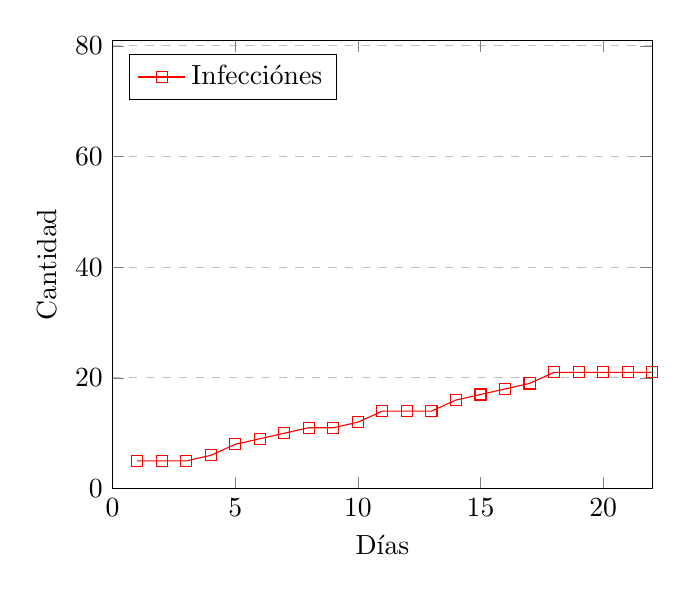
\begin{tikzpicture}
\begin{axis}[
xlabel={D\'ias},
ylabel={Cantidad},
xmin=0, xmax=22,
ymin=0, ymax=81,
legend pos=north west,
ymajorgrids=true,
grid style=dashed,
]
\addplot[
color=red,
mark=square,
]
coordinates {
(1, 5)(2, 5)(3, 5)(4, 6)(5, 8)(6, 9)(7, 10)(8, 11)(9, 11)(10, 12)(11, 14)(12, 14)(13, 14)(14, 16)(15, 17)(16, 18)(17, 19)(18, 21)(19, 21)(20, 21)(21, 21)(22, 21)
};
\legend{Infecci\'ones}
\end{axis}
\end{tikzpicture}
\newpage
\section{Cambios en el mapa}
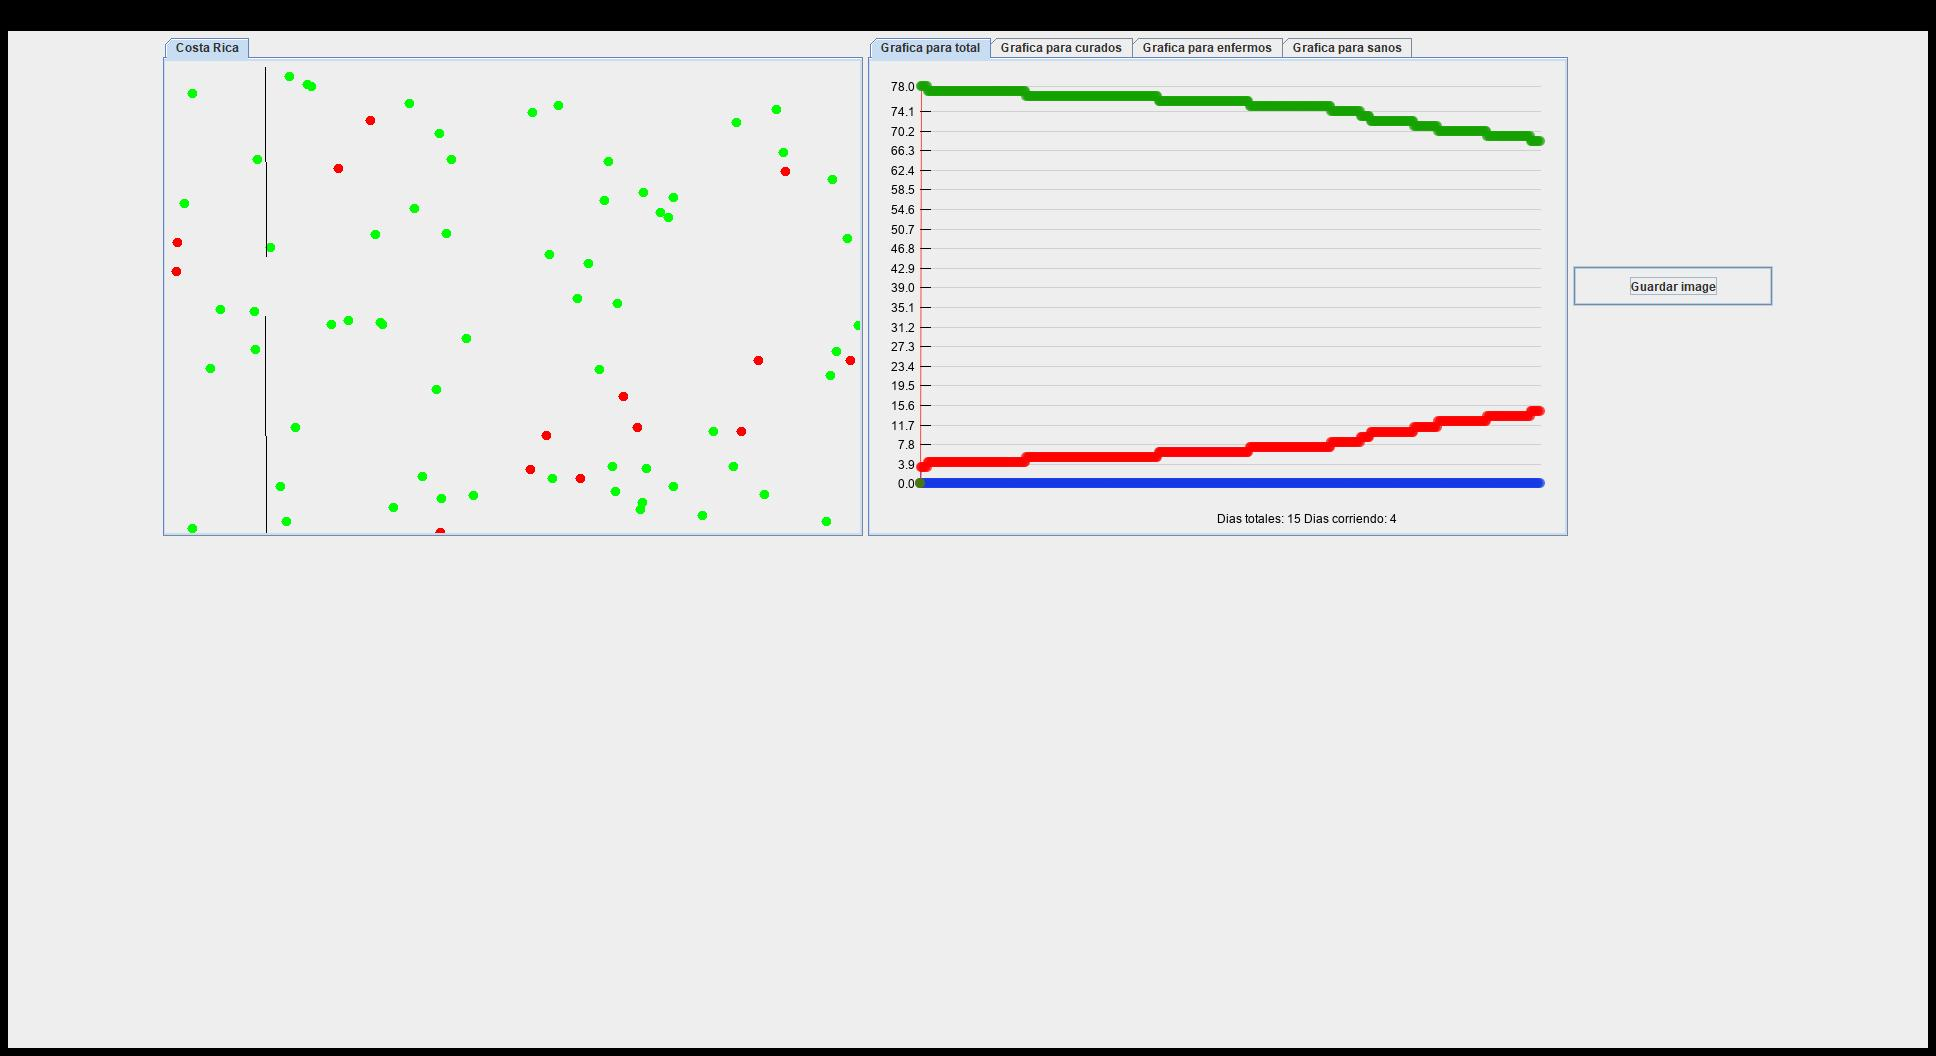
\includegraphics[scale=0.20]{grafica1.jpeg}
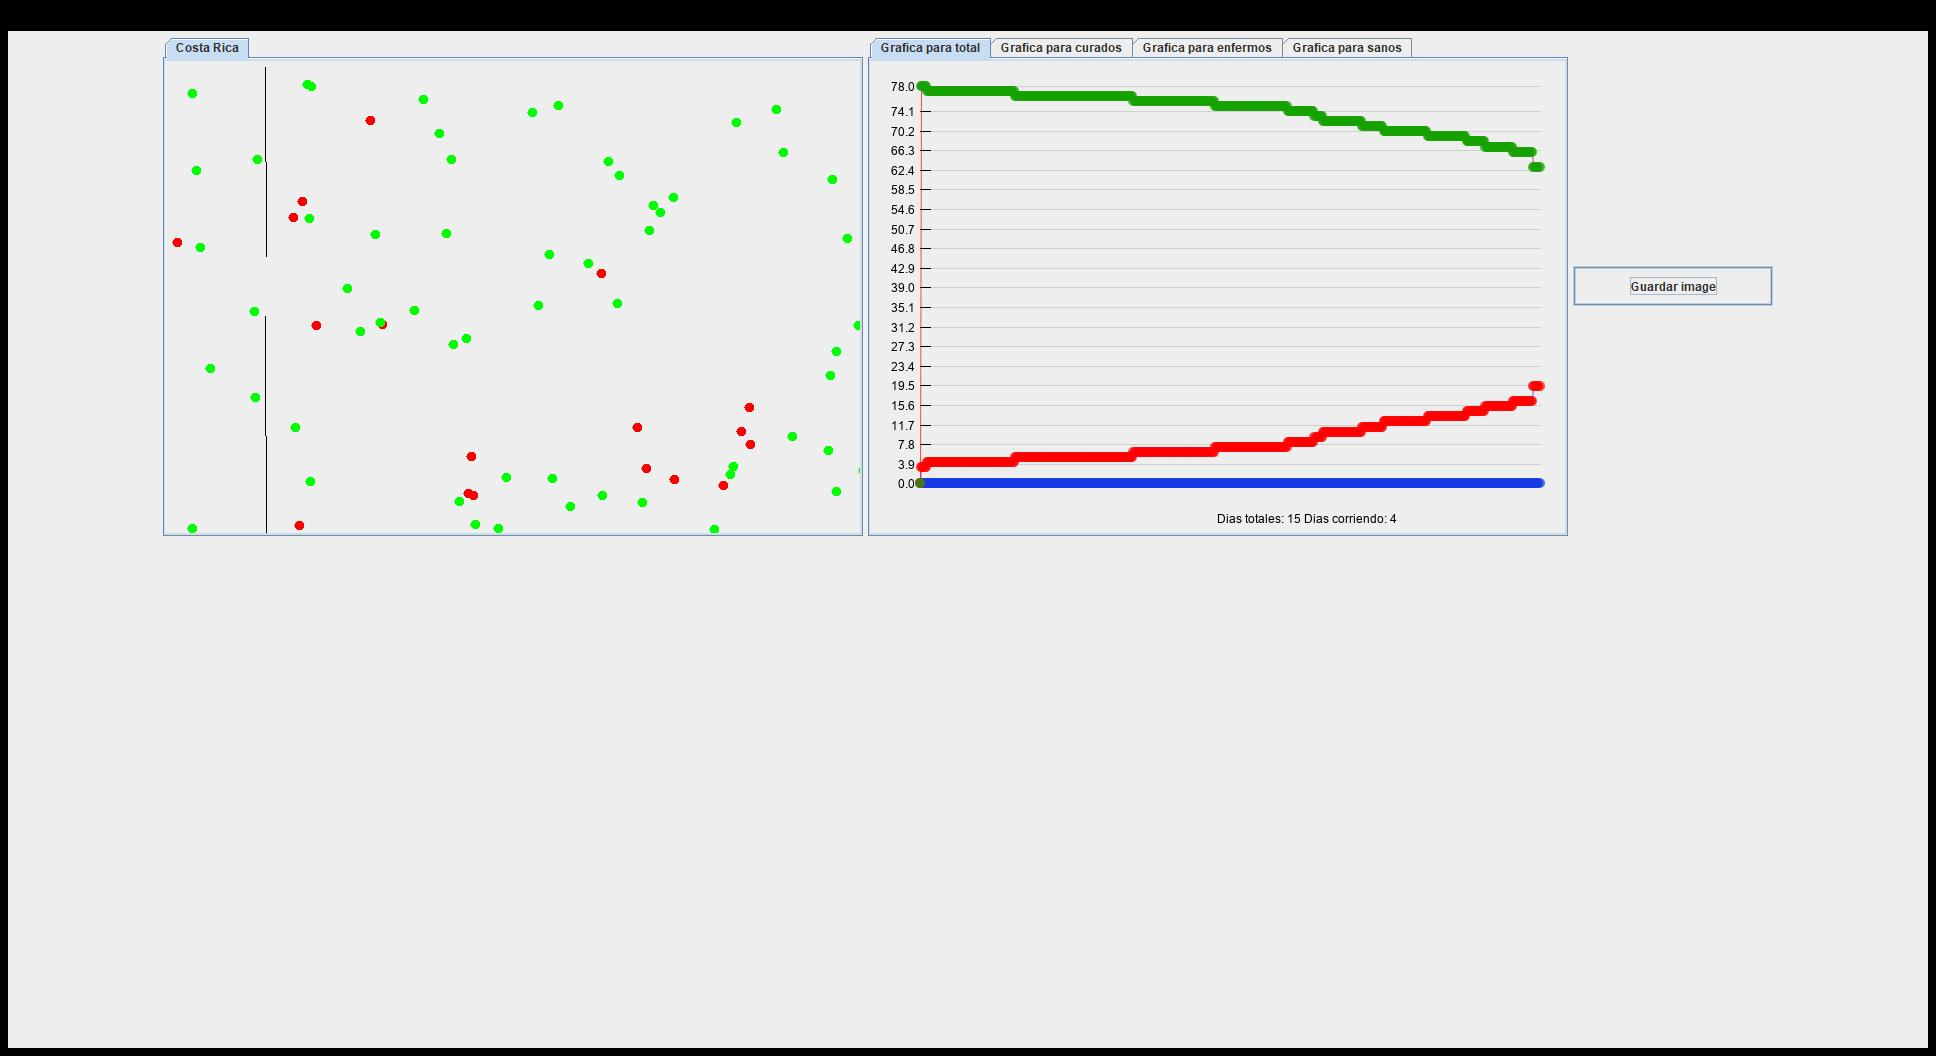
\includegraphics[scale=0.20]{grafica2.jpeg}
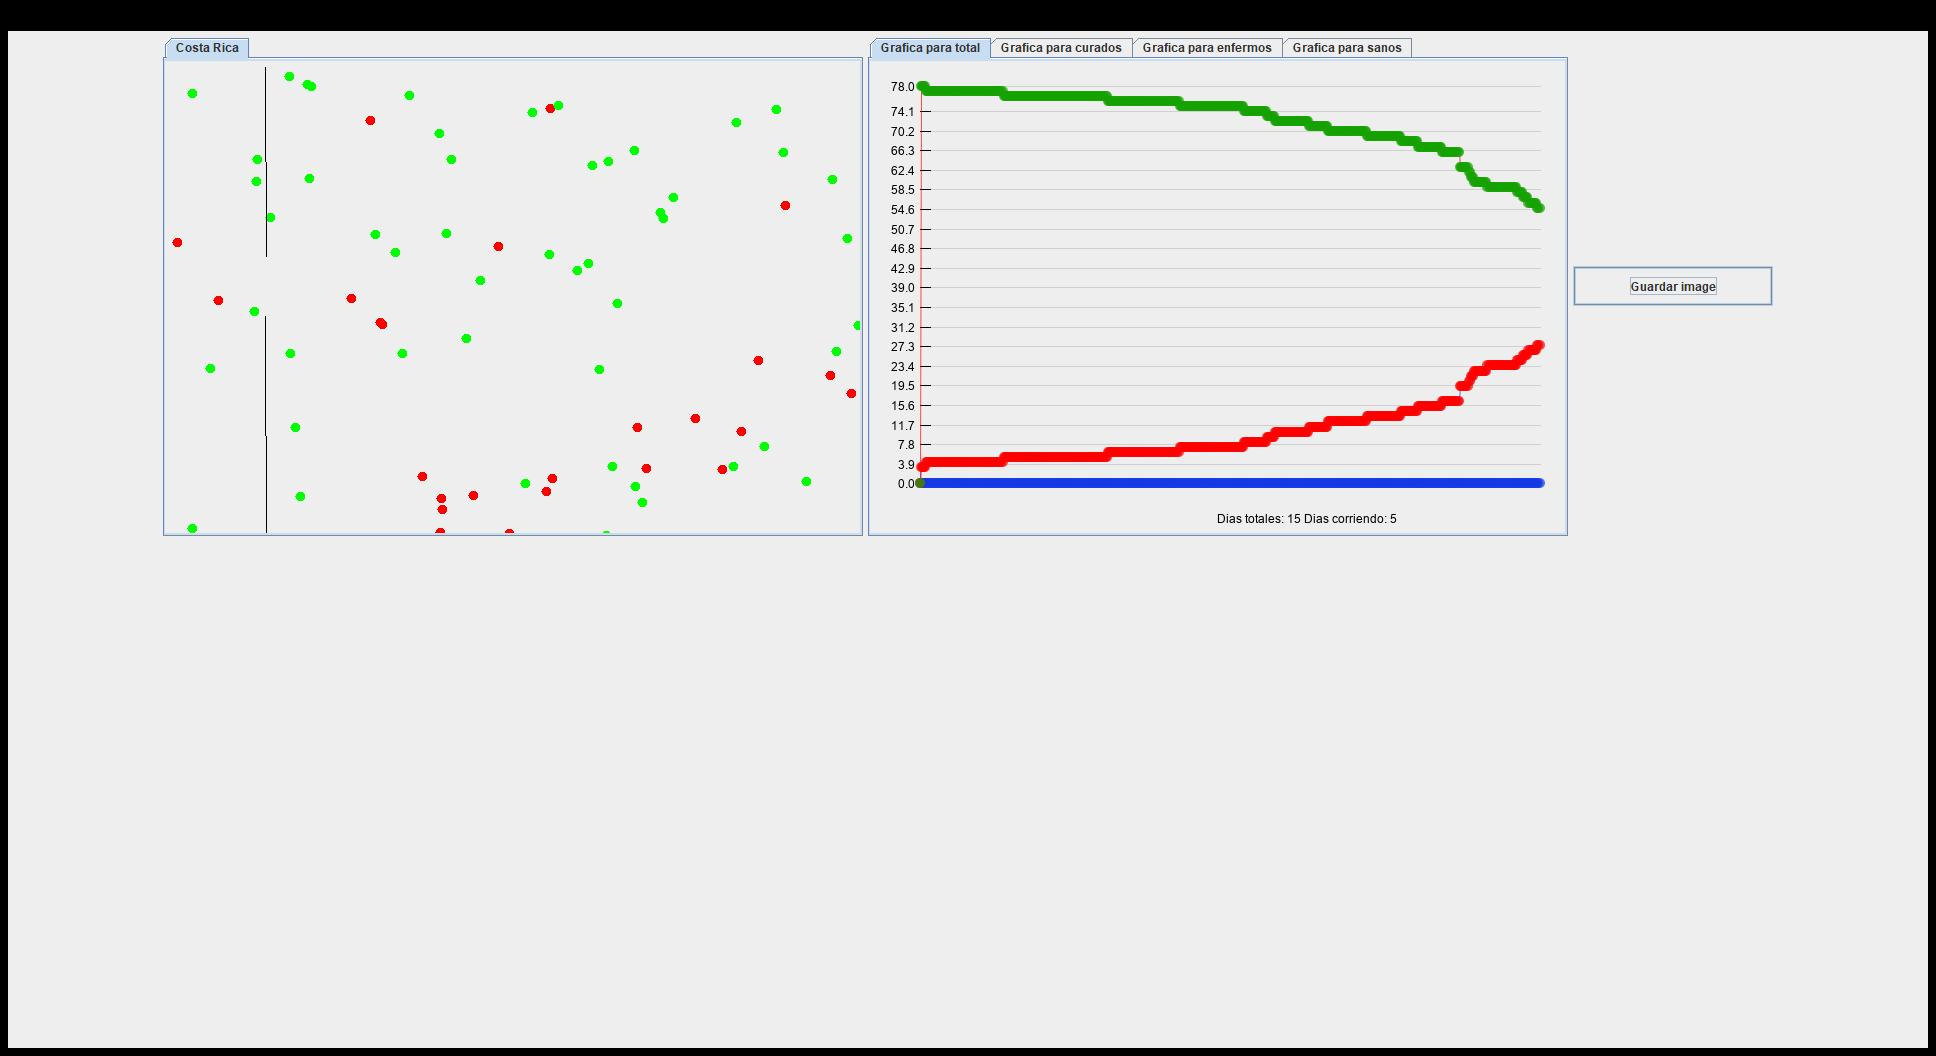
\includegraphics[scale=0.20]{grafica3.jpeg}
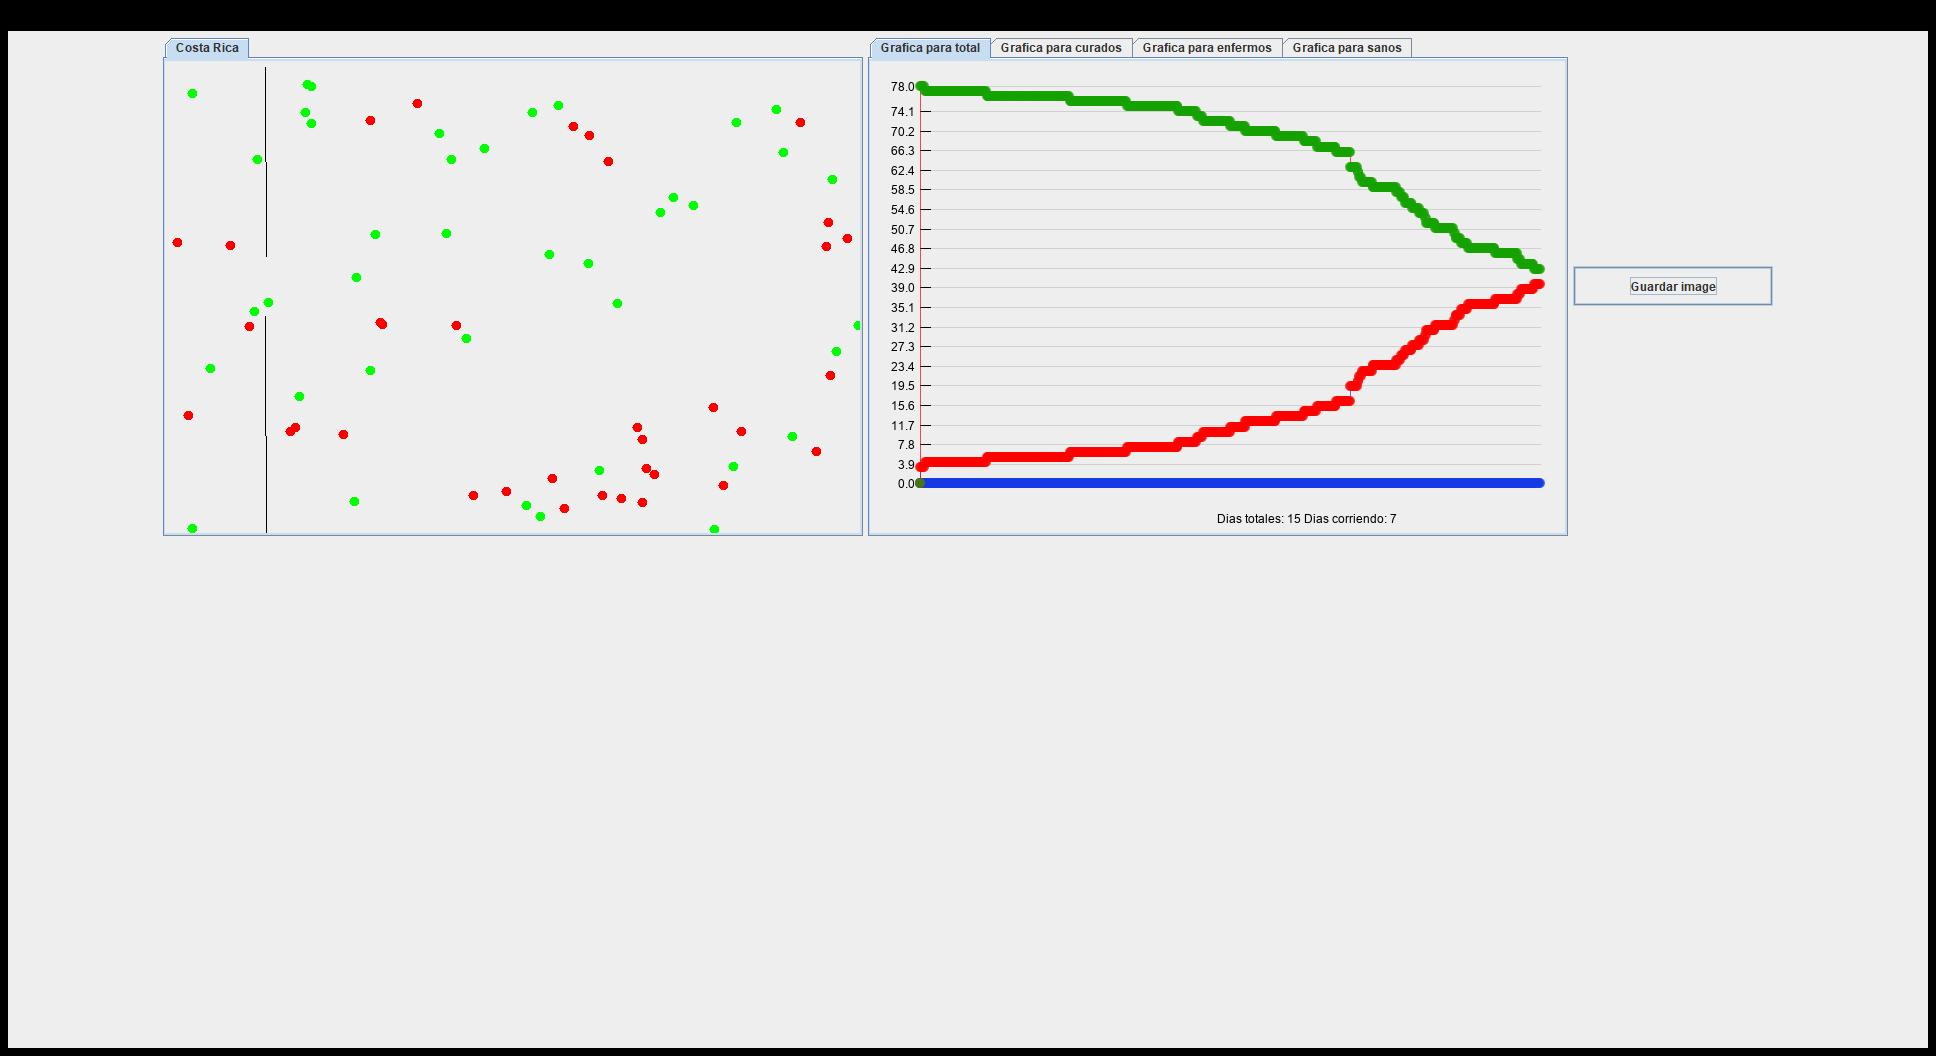
\includegraphics[scale=0.20]{grafica4.jpeg}
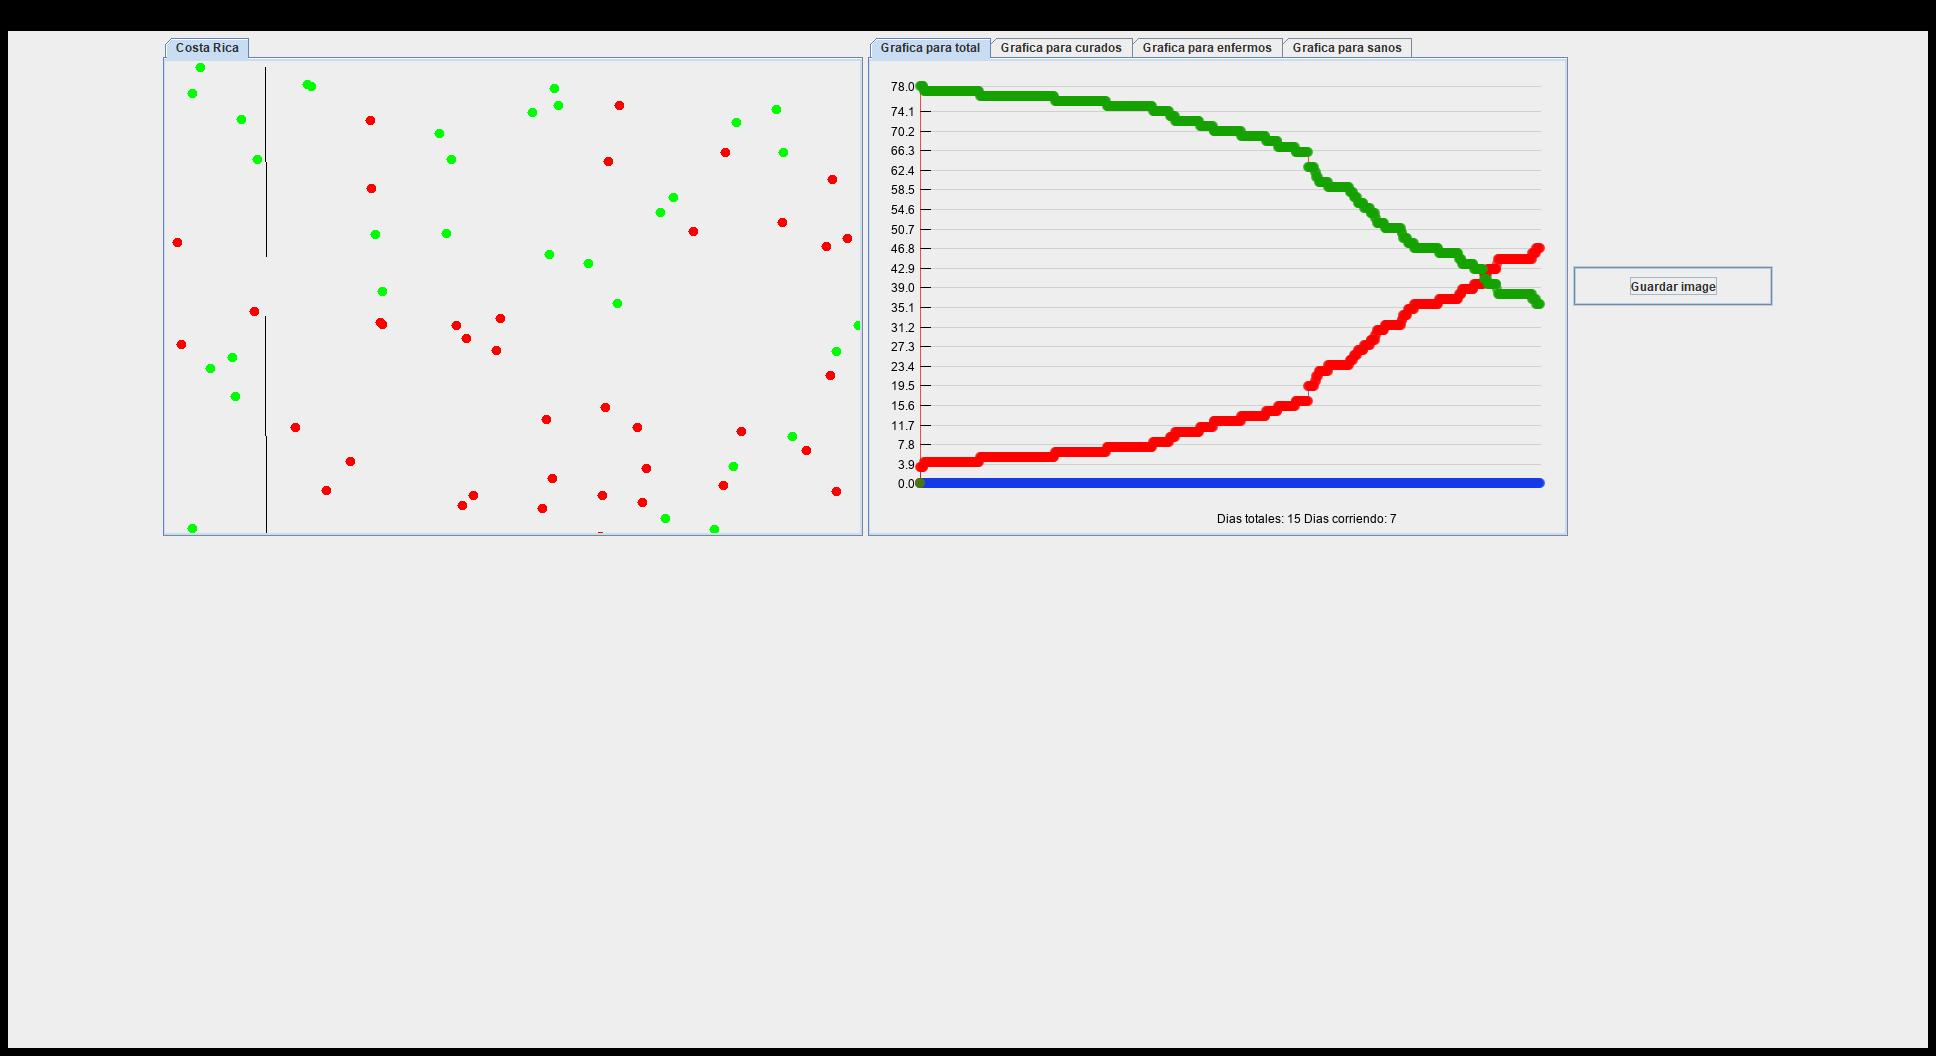
\includegraphics[scale=0.20]{grafica5.jpeg}
\end{document}
